\documentclass[11pt]{article}

\usepackage[margin=2.5cm]{geometry}
\usepackage{amsmath,amssymb}
\usepackage{graphicx}
\usepackage{booktabs}
\usepackage{caption}
\usepackage{subcaption}
\usepackage{hyperref}
\usepackage{enumitem}
\usepackage{array}
\usepackage{longtable}
\usepackage{xcolor}

\hypersetup{
  colorlinks=true,
  linkcolor=blue!45!black,
  citecolor=blue!45!black,
  urlcolor=blue!45!black
}

\newcommand{\msd}{\ensuremath{\langle x^2(t)\rangle}}
\newcommand{\code}[1]{\texttt{#1}}

\title{Inferring Collective Diffusion Regimes from Partial Agent Observation\\[4pt]
\large Project Report: Phases 1--3}
\author{}
\date{\today}

\begin{document}
\maketitle

\begin{abstract}
\noindent
This report documents three completed phases of a project that asks whether the
diffusion regime of a whole population of agents can be inferred from a small,
partially observed subset of them, using each observed agent's own trajectory
history together with the instantaneous mean field it experiences. Phase 1
builds and validates a toolbox of seven generative mechanisms and their
estimators and shows that a single trajectory can fail, in principle, to reveal
the population's exponent. Phase 2 quantifies exactly how estimators behave as a
function of trajectory length and turns mechanism identification into a
practical classification and bias-correction pipeline. Phase 3 couples agents
through a long-memory mean field and shows that coupling destroys a
superdiffusive agent's own signature but not a subdiffusive one, and separates
what a single agent can learn from what only the collective field reveals.
Phase 4 (heterogeneous sub-populations) has not been run; Phase 3's results are
its precondition.
\end{abstract}

\tableofcontents

% =====================================================================
\section{Introduction}
\label{sec:intro}

\subsection{Research question}

Given a population of agents whose microscopic motion rule is unknown, and
given access to only a subset of them, can the \textbf{diffusion regime of the
whole population} (subdiffusive, normal, or superdiffusive) be identified from
(i) an observed agent's own trajectory history and (ii) the instantaneous mean
field it experiences? The project attacks this question through four
sub-questions, in the order they are addressed:

\begin{description}[leftmargin=2.2em, style=nextline]
\item[Q1 --- Estimator quality.] For each generative mechanism, how well can
  the anomalous exponent be recovered from a single finite trajectory? Where
  does a single trajectory fail \emph{in principle} (ergodicity breaking)
  rather than merely from finite-sample noise?
\item[Q2 --- Mechanism discrimination.] Which observables separate mechanisms
  that share the same exponent (e.g.\ fractional Brownian motion vs.\
  continuous-time random walks vs.\ L\'evy walks)?
\item[Q3 --- Single agent vs.\ collective.] Once agents are coupled through a
  mean field, how correlated is a single agent's inferred regime with the
  ensemble's true regime? Does adding the mean-field signal as an extra
  observable help?
\item[Q4 --- Sampling cost under heterogeneity.] For a population made of $M$
  modules with different exponents, how many observed agents $n$ are needed to
  recover the population's exponent mixture, and how does the threshold ($\sim
  M$? $\sim M\log M$?) depend on the sampling strategy?
\end{description}

Phases 1--3 of this report answer Q1--Q3. Q4 is Phase 4 and has not been run;
Section~\ref{sec:conclusion} states what Phase 3 established as its
precondition.

\subsection{Background: anomalous diffusion and ergodicity breaking}

For an ensemble of independent trajectories, the ensemble-averaged mean
squared displacement scales as a power law in time, $\msd \sim t^\alpha$.
$\alpha=1$ is ordinary (Brownian) diffusion; $\alpha<1$ is \emph{subdiffusion}
(the population spreads slower than a random walk, typically because of
trapping or negatively correlated steps); $\alpha>1$ is
\emph{superdiffusion} (the population spreads faster, typically because of
long, persistent excursions). $\alpha$ is the single number this project spends
most of its effort trying to recover from limited data.

A subtlety drives half of this report: for some mechanisms, a single,
arbitrarily long trajectory does not reveal $\alpha$, even in principle. This
is \textbf{ergodicity breaking}. An ergodic process's \emph{time-averaged} mean
squared displacement (built from one trajectory, sliding a lag window along
it) converges to the same exponent as the \emph{ensemble-averaged} one
(built from many trajectories at fixed time) as the trajectory gets long.
A non-ergodic process's time-average does not converge to the ensemble
exponent --- it may converge to a different number entirely, or it may keep a
persistent, non-vanishing spread across realizations no matter how long the
trajectory runs. Whether a mechanism is ergodic, and what its time-average
does instead, is mechanism-specific and is one of the central facts Phase 1
establishes empirically (Table~\ref{tab:mechanisms}).

\subsection{Conventions that govern every result in this report}

Four rules, fixed before Phase 1 began, are load-bearing for everything that
follows and are stated here so later sections can rely on them without
re-deriving them:

\begin{itemize}
\item \textbf{Validation first.} A generator is not used for analysis until a
  test asserts that it reproduces its analytic ensemble MSD within a stated
  tolerance, over a stated time window. No result in this report comes from an
  unvalidated generator.
\item \textbf{Determinism.} Every stochastic function takes an explicit random
  number generator; there are no calls to hidden global random state. Every
  figure and every number in this report is reproducible from its
  configuration and seed.
\item \textbf{Fitting windows are explicit and asymmetric between two cases.}
  Power-law exponents are fitted by least squares on $\log(\mathrm{lag})$ or
  $\log(t)$ versus $\log(\mathrm{MSD})$, but \emph{time-averaged} MSD versus lag
  and \emph{ensemble-averaged} MSD versus time are not the same statistical
  claim and use different windows: the former is restricted to
  $[\mathrm{lag}_{\min}, T/10]$ because the number of independent lag windows
  collapses beyond that; the latter's window is instead an assertion about
  where the asymptotics of a specific mechanism hold, and is stated per case.
\item \textbf{Uncertainty comes from resampling particles, never from fit
  residuals.} Ensemble-averaged MSD points at different times are built from
  the same particles and are strongly correlated, so ordinary least-squares
  standard errors are not a valid confidence interval (Section~\ref{sec:phase1-bottlenecks}
  quantifies this by how much). Every reported uncertainty in this document is
  a bootstrap over particles or an empirical seed-to-seed spread.
\end{itemize}

% =====================================================================
\section{Phase 1 --- Single-agent and ensemble diffusion, no interaction}
\label{sec:phase1}

\subsection{Problem}

Phase 1 answers the foundational half of Q1 and Q2 without any coupling
between agents: build a library of generative mechanisms that covers the
qualitatively different ways a particle can diffuse anomalously, validate each
one against its analytic ensemble behaviour, build the estimator toolbox
needed to characterize a trajectory, and use both to answer, empirically:
\emph{how well does a single trajectory reveal the true exponent, and does
that answer depend on which mechanism generated the data?}

\subsection{Mechanisms studied}

Table~\ref{tab:mechanisms} lists the seven mechanisms implemented and
validated in Phase 1, together with the properties that distinguish them.
Two entries carry the most weight for the rest of the project. \textbf{CTRW}
(continuous-time random walk) is weakly ergodicity-breaking: its
time-averaged MSD grows \emph{linearly} in the lag regardless of the true
exponent $a$, and the amplitude of that linear growth is itself a random
variable that does not converge as the trajectory lengthens --- a single
trajectory cannot reveal $a$ no matter how long it runs. Its jump lengths are
Gaussian (finite variance), a deliberate choice: the point of contrasting CTRW
against fBm at $H<1/2$ is that they share an exponent but not an ergodic
property, and heavy-tailed jumps would blur that contrast into the L\'evy
walk. \textbf{L\'evy flight} has a diverging second moment, so MSD itself is
not a valid statistic for it; any code path that would compute one is made to
raise rather than silently return a finite number.

\begin{table}[htbp]
\centering
\caption{Generative mechanisms and their analytic signatures. $\alpha$ is the
ensemble MSD exponent, $\msd \sim t^\alpha$.}
\label{tab:mechanisms}
\begin{tabular}{lllccl}
\toprule
Mechanism & Regime & $\alpha$ & Ergodic & Gaussian prop.\ & Increment ACF \\
\midrule
Brownian & normal & $1$ & yes & yes & delta \\
fBm, $H<1/2$ & sub & $2H$ & yes & yes & negative \\
fBm, $H>1/2$ & super & $2H$ & yes & yes & positive \\
CTRW, $a\in(0,1)$ & sub & $a$ & \textbf{no} & no & zero + long pauses \\
L\'evy walk, $\gamma\in(1,2)$ & super & $3-\gamma$ & \textbf{no} & no & ballistic stretches \\
L\'evy flight, $s\in(0,2)$ & super & diverges & \textbf{no} & no (stable law) & delta \\
Scaled Brownian, $a$ & either & $a$ & \textbf{no} & yes & delta, non-stationary \\
Diffusing diffusivity & normal & $1$ & yes & \textbf{no} (exp.\ tails) & delta \\
\bottomrule
\end{tabular}
\end{table}

\subsection{Approach}

The pipeline is generators $\to$ validation $\to$ estimator toolbox $\to$
visualization, strictly in that order, because validation gates everything
downstream: no analysis is ever run on a generator that has not been checked
against its own analytic ensemble MSD. The estimator toolbox implements
time-averaged and ensemble-averaged MSD with power-law fitting, the
ergodicity-breaking parameter $\mathrm{EB}(\Delta)=\mathrm{Var}(\xi)$ with
$\xi=\overline{\delta^2}/\langle\overline{\delta^2}\rangle$, the van Hove
self-part (propagator shape), the increment autocorrelation, and the moment
scaling spectrum $\nu(q)$ (fit $\langle|x|^q\rangle\sim t^{q\nu(q)}$; a
piecewise-linear $\nu(q)$ with a kink is the L\'evy walk's fingerprint of
strong anomalous diffusion).

\subsection{Bottlenecks and how they were resolved}
\label{sec:phase1-bottlenecks}

\begin{itemize}
\item \textbf{Fit-residual error bars underestimate the true uncertainty by
  roughly 25$\times$.} The ensemble MSD is built from the same particles at
  every time point, so its points are strongly autocorrelated and ordinary
  least-squares standard errors are far too optimistic: measured over twelve
  seeds ($N{=}2000$, $T{=}1024$), the reported fit error was $\sim 0.0005$
  while the actual seed-to-seed standard deviation of the fitted exponent was
  $\sim 0.012$. This is why every uncertainty in this report is a bootstrap
  over particles, never \code{PowerLawFit.exponent\_err} (documented as a
  goodness-of-fit diagnostic only).
\item \textbf{CTRW's finite-time exponent bias changes sign with $a$.} The
  mean renewal count has a finite-time correction whose two terms pull in
  opposite directions: an additive $-1$ term biases the fitted exponent
  \emph{upward} at small $a$ (few renewals), while a slowly-decaying
  $(\tau_0/t)^{1-a}$ term biases it \emph{downward} as $a\to 1$. The measured
  bias at $T=4096$ runs $+0.069$ at $a=0.3$ down to $-0.071$ at $a=0.9$,
  crossing zero near $a\approx 0.6$ (later refined to $a=0.604$ at
  $T{=}4096$, drifting to $0.566$ by $T{=}65536$ --- the crossing itself is
  $T$-dependent). Consequence: a naive ``bias shrinks as $T$ grows'' test
  would be wrong, since the bias is a property of the observation window, not
  of the estimator alone.
\item \textbf{A log-space Jensen bias, found on review, was masquerading as
  part of the CTRW bias above.} A reviewer's independently-derived bias
  estimate ($+0.046$ at $a=0.3$) disagreed with the original ($+0.069$). The
  extra $+0.023$ turned out to be a genuine, separate effect: fitting
  $\log(\widehat{\mathrm{MSD}})$ introduces a bias of
  $-\sigma^2_{\mathrm{rel}}/2$ per Jensen's inequality, and because the
  CTRW's relative variance \emph{falls} with $t$ at small $a$, this tilts the
  log-log fit upward at finite ensemble size $N$. Measured at $a=0.3$,
  $T=4096$: bias $+0.067$ at $N{=}2000$, falling to $+0.042$ at $N{=}20000$,
  converging on the closed-form prediction of $+0.043$. This bias affects any
  log-log fit whose relative variance varies with the fitting abscissa, and
  bootstrapping gives a correct confidence interval but does not remove it.
\item \textbf{The L\'evy walk's MSD estimator gets noisier, not more precise,
  with time.} Because the fourth moment grows as $t^{5-\gamma}$, faster than
  the square of the second moment ($t^{6-2\gamma}$), the relative standard
  error of the ensemble MSD grows roughly as $t^{(\gamma-1)/2}$: measured at
  $\gamma=1.4$, $N=3000$, it runs from $1.9\%$ at $t=10$ to $5.7\%$ at
  $t=4095$. This is an independent reason (on top of the window-count
  argument) to cap the TA-MSD fitting window.
\item \textbf{Generators, not estimators, dominate memory.} At $N{=}4000$,
  $T{=}4096$ (one \code{float64} trajectory array is 125\,MiB), the L\'evy walk
  peaks at 1324\,MiB and fBm at 937\,MiB --- roughly $10\times$ and $7.5\times$
  the raw output array, from the event arrays and the complex FFT buffers
  respectively (Table~\ref{tab:benchmark}). Phase 2's sweeps generate in
  particle chunks rather than raising \code{n\_particles} directly.
\end{itemize}

\begin{table}[htbp]
\centering
\caption{Representative per-operation cost, $N{=}4000$, $T{=}4096$
(\code{results/benchmark\_table.json}).}
\label{tab:benchmark}
\begin{tabular}{lrr}
\toprule
Operation & Time (ms) & Peak memory (MiB) \\
\midrule
generate Brownian & 174 & 266 \\
generate fBm & 524 & 937 \\
generate SBM & 165 & 266 \\
generate CTRW & 1085 & 267 \\
generate L\'evy walk & 2157 & 1324 \\
generate L\'evy flight & 820 & 750 \\
generate diffusing diffusivity & 561 & 641 \\
TA-MSD (32 lags) & 1296 & 376 \\
EB curve (32 lags) & 1295 & 376 \\
moment spectrum (16 $q$) & 2234 & 250 \\
\code{fit\_powerlaw} (200 bootstrap) & 208 & 137 \\
\bottomrule
\end{tabular}
\end{table}

\subsection{Final result: the single-trajectory exponent table}

Table~\ref{tab:phase1-exponents} is Phase 1's closing measurement: 200
independent trajectories per mechanism per length, each fitted independently
on its own time-averaged MSD, at four lengths spanning a 64-fold range. The
column $p$ is the fitted exponent of $\mathrm{IQR}\sim T^{-p}$: a larger $p$
means the trajectory-to-trajectory spread shrinks faster as $T$ grows.

\begin{table}[htbp]
\centering
\caption{Single-trajectory TA-MSD exponent estimate, 200 trajectories per
cell (\code{results/exponent\_spread.json}). $p$ is the fitted IQR shrinkage
exponent, $\mathrm{IQR}\sim T^{-p}$.}
\label{tab:phase1-exponents}
\begin{tabular}{lccccccc}
\toprule
& & \multicolumn{4}{c}{Median $\hat\alpha$ ($T=$)} & & \\
\cmidrule(lr){3-6}
Mechanism & True $\alpha$ & 128 & 512 & 2048 & 8192 & $p$ \\
\midrule
Brownian & 1.00 & 0.958 & 0.976 & 0.997 & 0.990 & 0.263 \\
fBm, $H=0.3$ & 0.60 & 0.599 & 0.585 & 0.590 & 0.595 & 0.283 \\
Scaled Brownian, $a=0.6$ & 0.60 & 0.930 & 0.948 & 0.974 & 0.976 & 0.260 \\
CTRW, $a=0.5$ & 0.50 & 0.926 & 0.916 & 0.860 & 0.881 & 0.107 \\
Diffusing diffusivity & 1.00 & 0.966 & 0.972 & 0.987 & 0.991 & 0.264 \\
L\'evy walk, $\gamma=1.5$ & 1.50 & 1.622 & 1.522 & 1.489 & 1.472 & 0.050 \\
\bottomrule
\end{tabular}
\end{table}

Two qualitatively different failure modes sit inside this table, and the
distinction matters for Phase 2:

\begin{itemize}
\item \textbf{Scaled Brownian motion converges as tightly as Brownian motion,
  onto the wrong number.} Its IQR shrinks at essentially the ergodic rate
  ($p{=}0.260$, indistinguishable from Brownian's $p{=}0.263$), while its
  median walks toward $1.0$ against a true exponent of $0.6$. A single
  agent's own error bar gives no warning here: the estimate is precise and
  wrong.
\item \textbf{CTRW fails in the other direction}: the median is wrong
  \emph{and} the spread barely shrinks ($p{=}0.107$, roughly a third of the
  ergodic rate) --- both are the same non-ergodicity, showing up as bias in
  one statistic and as a stalled interquartile range in the other. CTRW and
  scaled Brownian motion both report $\hat\alpha\approx 1$ from one
  trajectory, for unrelated reasons (weak ergodicity breaking vs.\ ageing);
  that coincidence is the concrete form of the Q1 information wall, and it is
  exactly what makes single-trajectory mechanism classification hard --- the
  problem Phase 2 exists to address.
\end{itemize}

A second, independent check of the same non-ergodicity: for CTRW at
$a{=}0.5$, $N{=}2000$, $T{=}4096$, the measured ergodicity-breaking parameter
at lags $10/50/100$ is $0.700/0.866/1.009$ against a theoretical plateau of
$\pi/2-1=0.571$ --- systematically above the asymptotic plateau because
$\mathrm{EB}$ rises with $\mathrm{lag}/T$ and converges to the plateau only
slowly from above (Table~\ref{tab:ergodicity}, Figure~\ref{fig:ctrw-eb}).
Brownian motion's own EB, measured at the same lags, matches its closed form
$4\Delta/(3T)$ to within $5$--$9\%$ and serves as the positive control: a
plateau scaled by the wrong constant would still look like a plateau, but
this formula has a specific slope \emph{and} coefficient, and it is met.

\begin{table}[htbp]
\centering
\caption{Ergodicity-breaking parameter checks, $N{=}2000$, $T{=}4096$
(\code{results/ergodicity\_checks.json}).}
\label{tab:ergodicity}
\begin{tabular}{lrrrr}
\toprule
& \multicolumn{3}{c}{lag} & \\
\cmidrule(lr){2-4}
& 10 & 50 & 100 & target \\
\midrule
Brownian EB, measured & 0.00354 & 0.01734 & 0.03442 & \\
Brownian EB, predicted $4\Delta/(3T)$ & 0.00326 & 0.01628 & 0.03256 & \\
CTRW ($a{=}0.5$) EB, measured & 0.700 & 0.866 & 1.009 & plateau $0.571$ \\
\bottomrule
\end{tabular}
\end{table}

\subsection{Figures}

\begin{figure}[htbp]
\centering
\includegraphics[width=0.95\textwidth]{../results/media/phase1_figures/exponent_spread_all_mechanisms.png}
\caption{Single-trajectory exponent estimate vs.\ trajectory length $T$,
median and interquartile band, for six mechanisms
(\code{results/exponent\_spread.json}). Read off: Brownian, fBm and diffusing
diffusivity converge tightly onto their true exponent (dashed line); scaled
Brownian motion converges just as tightly but onto the \emph{wrong} number;
CTRW's band barely narrows and sits off-target; the L\'evy walk panel overlays
the naive OLS estimate against the flight-duration-MLE correction from Phase
2 (Section~\ref{sec:phase2-levy}), showing the correction pulling the band
down onto the true exponent.}
\label{fig:exponent-spread}
\end{figure}

\begin{figure}[htbp]
\centering
\includegraphics[width=0.75\textwidth]{../results/media/phase1_figures/ctrw_eb_vs_lag.png}
\caption{CTRW ergodicity-breaking parameter $\mathrm{EB}(\Delta)$ vs.\ lag,
$a{=}0.5$, $T{=}4096$. The curve sits above the theoretical plateau
($\pi/2-1=0.571$, dashed) and keeps rising with $\mathrm{lag}/T$ rather than
flattening within the plotted range --- the plateau is approached slowly from
above, not reached at any lag shown here.}
\label{fig:ctrw-eb}
\end{figure}

\begin{figure}[htbp]
\centering
\includegraphics[width=0.75\textwidth]{../results/media/phase1_figures/amplitude_scatter_ctrw_lag8.png}
\caption{Distribution of the normalized time-averaged-MSD amplitude
$\xi=\overline{\delta^2}/\langle\overline{\delta^2}\rangle$ at lag 8 across
2000 independent CTRW trajectories ($a{=}0.5$). An ergodic process would
concentrate this distribution at $\xi{=}1$; instead it has a finite density
at $\xi{\to}0$ (trajectories that spent the whole measurement inside one long
trapping event) and a heavy right tail. The measured $\mathrm{EB}{=}0.689$
sits close to its theoretical value $0.571$ for this one realization.}
\label{fig:amplitude-scatter}
\end{figure}

\begin{figure}[htbp]
\centering
\begin{subfigure}{0.48\textwidth}
\includegraphics[width=\textwidth]{../results/media/phase1_figures/van_hove_ctrw.png}
\caption{CTRW}
\end{subfigure}
\hfill
\begin{subfigure}{0.48\textwidth}
\includegraphics[width=\textwidth]{../results/media/phase1_figures/van_hove_ddm.png}
\caption{Diffusing diffusivity}
\end{subfigure}
\caption{Self-part of the van Hove distribution $G_s(\Delta x, t)$ at several
times, versus a Gaussian reference (dashed). CTRW develops a sharp central
peak and non-Gaussian tails driven by particles still trapped in their first
waiting interval; diffusing diffusivity keeps a symmetric but sub-Gaussian
central peak with exponential (not Gaussian) tails at short times, the
signature of a fluctuating local diffusion coefficient. Both mechanisms have
$\alpha=1$ at the level of the MSD alone --- the propagator shape is what
separates them, motivating the feature set Phase 2 builds on.}
\label{fig:van-hove}
\end{figure}

\begin{figure}[htbp]
\centering
\includegraphics[width=0.75\textwidth]{../results/media/phase1_figures/increment_acf.png}
\caption{Increment autocorrelation $\rho(k)$ for five configurations, against
the closed-form fBm prediction (dashed). Brownian motion and CTRW are
indistinguishable at $\rho(k)=0$ for $k\geq1$ (delta-correlated increments);
fBm at $H{=}0.3$ dips negative at lag 1 (antipersistence) while $H{=}0.7$
stays positive and decays slowly (persistence); the L\'evy walk's increments
stay strongly positively correlated out to lag 10, the ballistic-stretch
signature.}
\label{fig:increment-acf}
\end{figure}

\begin{figure}[htbp]
\centering
\begin{subfigure}{0.48\textwidth}
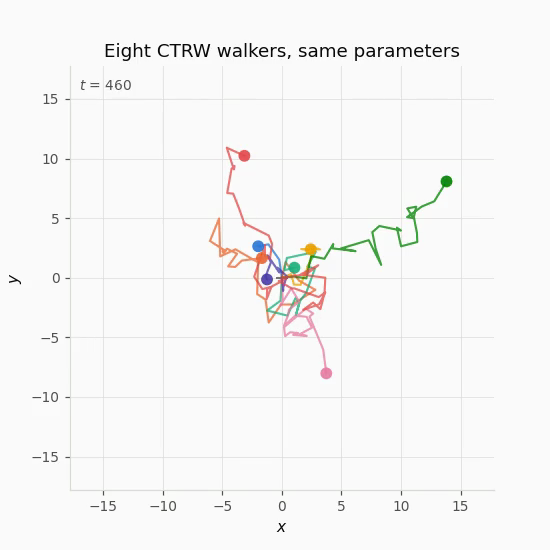
\includegraphics[width=\textwidth]{figs/ctrw_few_still.png}
\caption{Eight independent CTRW walkers, same parameters (frame from
\code{results/media/ctrw\_few.mp4}).}
\end{subfigure}
\hfill
\begin{subfigure}{0.48\textwidth}
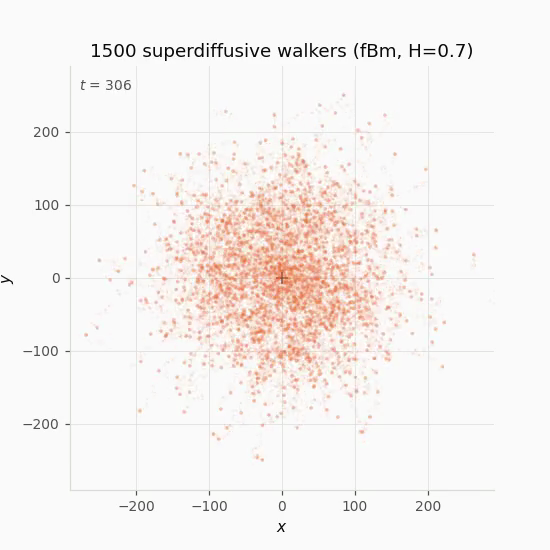
\includegraphics[width=\textwidth]{figs/fbm_cloud_still.png}
\caption{1500 superdiffusive walkers, fBm $H{=}0.7$ (frame from
\code{results/media/fbm\_cloud.mp4}).}
\end{subfigure}
\caption{Representative stills from the trajectory animations regenerated in
this report's re-run. The CTRW panel shows the qualitative signature of weak
ergodicity breaking directly: walkers alternate between long flat pauses and
short jumps, so different realizations of ``the same process'' visibly cover
very different territory in the same elapsed time --- the trajectory-level
picture behind Table~\ref{tab:phase1-exponents}'s CTRW row.}
\label{fig:trajectories}
\end{figure}

\clearpage
% =====================================================================
\section{Phase 2 --- Estimator identifiability}
\label{sec:phase2}

\subsection{Problem}

Given a trajectory length $T$ and an ensemble size $N$, what is the bias and
variance of each estimator, per mechanism, and can mechanisms that share an
exponent be told apart from a single trajectory at all? This is Q1 made
quantitative and Q2 made operational.

\subsection{Approach}

Phase 2 builds 19 scale-invariant features (invariant under $x\mapsto cx$,
verified for every feature on every mechanism) grouped into seven families
(TA-MSD shape, increment ACF, non-Gaussian parameter, immobility, $p$-variation,
excursion, non-stationarity; Table~\ref{tab:features}), trains pairwise and
multi-class classifiers on them, compares a Whittle (spectral maximum
likelihood) estimator against Phase 1's naive TA-MSD fit relative to the
Cram\'er--Rao bound, and closes the loop with a conditional exponent-correction
pipeline: classify the mechanism, then apply a mechanism-specific bias
correction before reporting $\hat\alpha$.

\begin{table}[htbp]
\centering
\caption{Feature families used for mechanism classification, $T\in\{128,
512, 2048, 8192\}$, 120 trajectories per mechanism per length, 6 mechanisms
(\code{results/phase2/step2\_dataset\_summary.json}).}
\label{tab:features}
\begin{tabular}{ll}
\toprule
Family & Representative features \\
\midrule
\code{tamds} & TA-MSD fitted exponent, TA-MSD ratio \\
\code{acf} & increment autocorrelation at lags 1, 2, 3, 5, 10 \\
\code{ngp} & non-Gaussian parameter at lags 1, 5, 10 \\
\code{immobility} & immobile fraction, mean/max gap length \\
\code{p\_variation} & $p$-variation ratios at $p{=}1,2,3$ \\
\code{excursion} & maximal excursion ratio, range-to-std ratio \\
\code{nonstationarity} & increment variance ratio (early vs.\ late) \\
\bottomrule
\end{tabular}
\end{table}

\subsection{Bottleneck told in full: the L\'evy-walk exponent correction}
\label{sec:phase2-levy}

The conditional-correction pipeline initially fell through to Phase 1's naive
TA-MSD fit for the L\'evy walk regardless of whether the mechanism was known
or predicted --- a review flagged that \code{mae\_naive}, \code{mae\_oracle}
and \code{mae\_predicted} were bit-identical for that one mechanism in
\code{step6\_conditional\_exponent.json}. Three approaches were tried before
one worked.

\begin{enumerate}
\item \textbf{GLS-weighted TA-MSD fit (failed).} \code{PROJECT.md}'s own
  fitting convention prescribes bootstrapping the lag--lag covariance of
  $\log(\mathrm{TA\text{-}MSD})$ and weighting the log-log fit by its inverse.
  Tried four ways (full covariance with ridge regularization, diagonal-only
  inverse variance, rank-truncated pseudo-inverse, and a control using the
  \emph{true} ensemble covariance from 800 independent trajectories). Every
  variant was worse than plain OLS; the true-covariance control was
  dramatically worse ($\mathrm{MAE}\approx 0.43$ vs.\ naive's
  $\approx 0.13$). Diagnosis: a single trajectory's short lags are precise but
  biased toward the ballistic within-flight regime, while its long lags are
  asymptotically correct but individually noisy. Inverse-variance weighting
  does exactly what it is built to do and concentrates weight on the
  precise-but-biased end, making the bias worse rather than better --- a
  mismatch between the weighting objective (minimize variance) and the actual
  failure mode (lag-dependent bias), not a bootstrap-implementation bug.
\item \textbf{Moment-spectrum kink fit (failed).} The moment spectrum
  $\nu(q)$ is the L\'evy walk's textbook fingerprint, but resolving its
  high-$q$ branch needs an ensemble, which one trajectory does not have.
  Direct single-trajectory fit: $\mathrm{MAE}\approx 0.41$. Building a
  pseudo-ensemble by splitting one trajectory into 16--192 segments and
  sweeping the segment count and fit window did better but plateaued at
  $\mathrm{MAE}\approx 0.147$--$0.15$, still worse than naive's $\approx 0.13$.
\item \textbf{Flight-duration MLE via sub-grid reconstruction (adopted).}
  Both prior attempts reweighted or refit a statistic \emph{derived} from the
  trajectory. Instead, mirroring the CTRW correction (which already works by
  doing MLE directly on waiting-time durations), flight durations are
  reconstructed from the gridded trajectory: flight speed is estimated as
  $\max(|{\rm diff}|)$, each grid step is classified as ``pure'' (interior to
  one flight) or ``straddling'' (containing a turning point), and a
  straddling step's fractional turning time is solved exactly from its one
  displacement value once neighbouring pure steps fix the flight directions.
  This sub-grid resolution matters because $\tau_0$ is order-1, the same
  order as the grid spacing $dt$, so a large fraction of true flights are
  shorter than one grid step. A Hill estimator on the upper tail of the
  reconstructed durations gives a tail index $\hat\gamma$; the final
  exponent blends the naive fit and the correction,
  $w\,\hat\alpha_{\rm naive} + (1-w)(3-\hat\gamma)$, rather than trusting the
  Hill estimate alone (its reliability depends on the flight count, which
  shrinks as $\gamma\to1$). A ceiling check --- a Pareto MLE on the
  \emph{true}, unquantized event durations --- reaches $\mathrm{MAE}\approx
  0.05$ against naive's $\approx 0.13$, confirming the signal is real; the
  practical grid-reconstructed version recovers part of it.
\end{enumerate}

\textbf{Tuning pitfall.} The first tuning pass fixed $\tau_0{=}\mathrm{speed}{=}1$
and found $w{=}0.6$, $\mathrm{top\_frac}{=}0.4$ cut MAE by $\sim20\%$,
validated across 8 seeds. Re-running with the actual sampling distribution
($\tau_0,\mathrm{speed}\sim U(0.5,2.0)$) showed almost no improvement
($0.1161\to0.1163$): a varying $\tau_0$ weights the harder-to-reconstruct
short-flight regime more heavily than the fixed-$\tau_0$ tuning set did, and
the first-pass parameters had overfit to the easier case. Retuning against
600 realistically-drawn trajectories ($w{=}0.6$,
$\mathrm{top\_frac}{=}0.35$) gave a held-out improvement of $0.133\to0.121$
($\sim9\%$). \textbf{Lesson: tune and validate against the actual
parameter-generating distribution, not a convenient fixed-parameter subset of
it} --- one additional free parameter changed which correction looked best.

\subsection{Final results}

Table~\ref{tab:classification} shows multi-class classification accuracy
(gradient boosting, the best of three classifiers tried) as a function of
trajectory length, and Table~\ref{tab:pairwise} shows the three
hardest-to-separate mechanism pairs individually. \code{fBm} vs.\ \code{CTRW}
--- the pair chosen specifically because they share an exponent but not an
ergodic property --- separates completely at every length tested; ablation
confirms that \code{immobile\_fraction} alone achieves $100\%$ pairwise
accuracy. \code{SBM} vs.\ \code{Brownian} separates only asymptotically,
improving steadily as $T$ grows. \code{DDM} vs.\ \code{Brownian} is already
well separated by $T{=}128$ via the non-Gaussian parameter, which is the
short-time signature of a fluctuating diffusivity.

\begin{table}[htbp]
\centering
\caption{Six-way mechanism classification accuracy, gradient boosting
classifier (\code{results/phase2/step3\_classification\_summary.json}).
``Interp.'' trains and tests on the same length; ``extrap.'' trains on a
pooled set and tests on held-out trajectories of that length.}
\label{tab:classification}
\begin{tabular}{lcc}
\toprule
$T$ & Interp.\ accuracy & Extrap.\ accuracy \\
\midrule
128 & 0.747 & 0.786 \\
512 & 0.861 & 0.913 \\
2048 & 0.928 & 0.963 \\
8192 & 0.961 & 0.950 \\
\bottomrule
\end{tabular}
\end{table}

\begin{table}[htbp]
\centering
\caption{Pairwise classification error for the three hardest-to-separate
mechanism pairs (\code{results/phase2/step3\_classification\_summary.json},
\code{step4\_ablation\_summary.json}).}
\label{tab:pairwise}
\begin{tabular}{lcccc}
\toprule
Pair & $T{=}128$ & $T{=}512$ & $T{=}2048$ & $T{=}8192$ \\
\midrule
fBm vs.\ CTRW & 0.000 & 0.000 & 0.000 & 0.000 \\
SBM vs.\ Brownian & 0.296 & 0.208 & 0.100 & 0.050 \\
DDM vs.\ Brownian & 0.025 & 0.000 & 0.000 & 0.000 \\
\bottomrule
\end{tabular}
\end{table}

Feature ablation at $T{=}2048$ (baseline accuracy $0.928$) shows the
non-Gaussian-parameter and non-stationarity families carry the most
irreplaceable information: removing \code{ngp} drops accuracy to $0.839$ and
removing \code{nonstationarity} to $0.857$, while removing any other single
family costs less than one percentage point (Table~\ref{tab:ablation}). At
the single-feature level, \code{immobile\_fraction} alone reaches $100\%$
accuracy on fBm-vs-CTRW and \code{ngp\_lag1} alone reaches $100\%$ on
DDM-vs-Brownian --- each pair has one feature that is, on its own, already
sufficient.

\begin{table}[htbp]
\centering
\caption{Leave-one-family-out ablation, gradient boosting, $T{=}2048$
(\code{results/phase2/step4\_ablation\_summary.json}). Lower accuracy after
removal means the family mattered more.}
\label{tab:ablation}
\begin{tabular}{lc}
\toprule
Configuration & Accuracy \\
\midrule
Full feature set (baseline) & 0.928 \\
without \code{ngp} & 0.839 \\
without \code{nonstationarity} & 0.857 \\
without \code{acf} & 0.922 \\
without \code{immobility} & 0.922 \\
without \code{tamds} & 0.929 \\
without \code{excursion} & 0.929 \\
without \code{p\_variation} & 0.932 \\
\bottomrule
\end{tabular}
\end{table}

Table~\ref{tab:whittle} compares Phase 1's naive TA-MSD fit against a Whittle
(spectral) maximum-likelihood estimator, relative to the Cram\'er--Rao lower
bound, for fBm at $H{=}0.3$ and $H{=}0.7$. The Whittle estimator is close to
asymptotically efficient by $T{=}8192$; the naive estimator's efficiency
\emph{falls} as $T$ grows, showing its spread is a limitation of the
estimator, not of the information present in the data.

\begin{table}[htbp]
\centering
\caption{Estimator efficiency relative to the Cram\'er--Rao bound
(\code{results/phase2/step5\_information\_floor.json}).}
\label{tab:whittle}
\begin{tabular}{lcccc}
\toprule
& \multicolumn{4}{c}{Efficiency at $T=$} \\
\cmidrule(lr){2-5}
& 128 & 512 & 2048 & 8192 \\
\midrule
$H{=}0.3$, naive TA-MSD & 0.448 & 0.320 & 0.227 & 0.094 \\
$H{=}0.3$, Whittle MLE & 0.779 & 0.813 & 0.743 & 0.968 \\
$H{=}0.7$, naive TA-MSD & 0.289 & 0.163 & 0.063 & 0.036 \\
$H{=}0.7$, Whittle MLE & 0.568 & 0.556 & 0.568 & 0.704 \\
\bottomrule
\end{tabular}
\end{table}

Finally, Table~\ref{tab:exponent-mae} closes the loop: naive
Phase-1-style fitting, prediction-corrected fitting (classify, then apply the
mechanism-specific correction, including the L\'evy-walk correction above),
and an oracle that already knows the true mechanism, at $T{=}2048$. The
correction pipeline cuts overall MAE by $68.8\%$
($0.1687\to0.0527$), most of the way to the oracle's $0.0478$; the residual
gap of $0.0049$ is the cost of occasionally misclassifying the mechanism.

\begin{table}[htbp]
\centering
\caption{Exponent recovery MAE by mechanism, $T{=}2048$
(\code{results/phase2/step6\_conditional\_exponent.json}).}
\label{tab:exponent-mae}
\begin{tabular}{lccc}
\toprule
Mechanism & Naive & Predicted & Oracle \\
\midrule
Brownian & 0.0532 & 0.0028 & 0.0000 \\
fBm & 0.0619 & 0.0272 & 0.0206 \\
CTRW & 0.3519 & 0.0906 & 0.0906 \\
SBM & 0.3654 & 0.0761 & 0.0627 \\
DDM & 0.0634 & 0.0064 & 0.0000 \\
L\'evy walk & 0.1161 & 0.1132 & 0.1132 \\
\midrule
\textbf{Overall} & \textbf{0.1687} & \textbf{0.0527} & \textbf{0.0478} \\
\bottomrule
\end{tabular}
\end{table}

No figures accompany Phase 2 in the current repository: its results are
tables and JSON summaries rather than saved plots, so they are reported
here as tables only, per this report's sourcing rule.

\clearpage
% =====================================================================
\section{Phase 3 --- Mean-field coupling}
\label{sec:phase3}

\subsection{Problem}

Once agents are coupled through a mean field, how much does a single agent's
inferred regime tell you about the true collective regime, and does the
field help (Q3)? This requires a coupled model with a well-defined
``collective regime,'' a validated way to measure both the agent-level and
field-level exponent, and a comparison of observers that do and do not use the
field.

\subsection{Model}

Each agent's velocity follows the AR($\infty$) representation of an
ARFIMA$(0,d,0)$ process, truncated at $K$ lags, with consensus coupling to the
instantaneous mean field:
\[
v_i(t+1) = \sum_{s=1}^{K}\kappa(s)\,v_i(t+1-s) \;+\; J\big(\langle v\rangle(t) - v_i(t)\big) \;+\; \sigma\,\eta_i(t+1),
\qquad
\kappa(s) = \frac{\Gamma(s-d)}{\Gamma(-d)\Gamma(s+1)}.
\]
The consensus form $J(\langle v\rangle - v_i)$, not an additive $+J\langle
v\rangle$, is essential: because $\sum_s\kappa(s)=1$, the additive form would
make the collective mode unstable for any $J>0$. With consensus coupling, the
$J$ term cancels exactly under all-to-all averaging, so the mean field
$\langle v\rangle(t)$ is itself exactly ARFIMA$(0,d,0)$ with variance
$\sigma^2/N$, \emph{for every value of $J$} --- the \textbf{conservation law}
this phase's validation is built around. The shared asymptotic exponent is
\[
\alpha = 1+2d, \qquad d\in(-\tfrac12,\tfrac12).
\]

The deviation from the mean field, $\delta_i=v_i-\langle v\rangle$, has a
closed-form spectrum
$S_\delta(\omega) = \sigma^2 / \big|(1-e^{-i\omega})^d + Je^{-i\omega}\big|^2$,
and its low-frequency behaviour depends on the \textbf{sign of $d$}:

\begin{itemize}
\item $d>0$ (superdiffusive memory): the denominator tends to $J$ as
  $\omega\to0$, so $S_\delta(0)=\sigma^2/J^2$ is finite --- the deviation
  becomes ordinary diffusion at long times, with memory surviving only below
  a crossover $\tau_c\sim J^{-1/|d|}$.
\item $d<0$ (subdiffusive memory): the fractional term diverges as
  $\omega\to0$ and dominates $J$ at every reachable frequency,
  $S_\delta(\omega)\sim\omega^{2|d|}\to0$. Coupling does \emph{not} destroy
  the anomalous exponent, and $\tau_c$ has no meaning.
\end{itemize}

This is the section's central physical result, stated plainly:
\textbf{coupling kills superdiffusive memory but not subdiffusive memory.}
Whether an isolated single-agent observer can still reach the true collective
regime depends on which side of zero $d$ is on.

\subsection{Bottlenecks, told as a sequence}

This phase had the most iterations of any in the project; each one changed
what could legitimately be measured next.

\begin{description}[leftmargin=1.4em, style=nextline]
\item[V1: wrong reference process.] The original specification claimed the
  $J{=}0$ limit was exactly fractional Gaussian noise (fGn). Validating
  against fGn's closed-form autocorrelation showed a persistent gap
  ($\sim0.08$--$0.09$ at lag 1) that did \emph{not} shrink between $K{=}64$
  and $K{=}1024$, ruling out ordinary truncation error. The correct reference
  is ARFIMA$(0,d,0)$, not fGn: the two share the asymptotic exponent
  $\alpha{=}1{+}2d$ but not the short-lag correlation
  ($\rho(1)=d/(1-d)$ for ARFIMA vs.\ $2^{2d}-1$ for fGn). Re-validating
  against the corrected target dropped the maximum deviation from $\sim0.08$
  to $0.005$--$0.007$ (Table~\ref{tab:v1}) --- the simulator was correct all
  along; the specification's reference process was not.
\item[V2/V3: sweep recalibration and a normalization bug.] The default $J$
  grid predicted $\tau_c$ values spanning 16 to 160{,}000 at $d{=}0.25$, only
  one of which fell inside the trustworthy $K/10$ window; the grid was
  replaced with one targeted directly at $\tau_c\in\{8,16,32,64\}$. The
  deviation-spectrum validation (V3) then showed the simulator and the
  closed-form spectrum agreeing in shape but differing by a flat factor of
  $2\pi$ --- a missing normalization constant in the spectral-density
  formula, fixed, after which the mean absolute log-ratio in the trustworthy
  band fell to $0.036$--$0.037$ (Table~\ref{tab:v3}).
\item[V4: redesigned from a crossover measurement to a joint fit.] The first
  attempt to locate $\tau_c$ from the local slope of an agent's own MSD gave
  a slope of $\log\tau_c$ vs.\ $\log J$ of $+1.09$ against a predicted
  $-4.0$ --- wrong sign, and not fixable by averaging more realizations. The
  diagnosis: the recalibrated $J$ grid makes $J$ comparable to or larger
  than $\kappa(1)=d$, so the local-slope measurement was probing a regime the
  low-frequency crossover argument was never actually valid for --- it is not
  that the measurement failed, it is that nothing predicted it should
  succeed. V4 was redesigned as a joint $(d,J)$ Whittle MLE against the
  deviation spectrum instead, which fits the whole spectral shape rather than
  one feature of it (Table~\ref{tab:v4}). An optimizer bug was found en
  route: a single L-BFGS-B run from the bounds' midpoint converged to a poor
  local optimum whenever the true $J$ was far from that midpoint (most of the
  grid); fixed with a $3\times3$ multi-start grid. The original crossover
  measurement is kept only as a qualitative illustration
  (Figure~\ref{fig:crossover}), explicitly not asserted as a measurement.
\item[Step 2: a naive, coupling-blind Whittle fit is misleading for $d<0$.]
  Fitting the correct, coupling-aware two-parameter model recovers the true
  $d$ regardless of $J$ by construction --- informative for Q3's
  model-aware observer, but useless for \emph{demonstrating} the
  phenomenological crossover this step exists to show. A coupling-blind,
  one-parameter Whittle fit shows the expected decline for $d>0$, but
  \emph{also} declines sharply for $d<0$ (contradicting the ``subdiffusive
  memory survives'' prediction): the $+Je^{-i\omega}$ term reshapes the whole
  spectrum, not just its low-frequency limit, so forcing a one-parameter
  model onto genuinely two-parameter data biases the fit regardless of the
  true sign of $d$. Resolved by using a model-free, windowed
  ensemble-averaged MSD fit as the primary ``typical-agent'' measure instead
  --- it cannot inherit a spectral model's misspecification because it
  assumes no spectral model at all.
\item[Close-out: two field-side Whittle bugs, found late, that silently
  changed earlier numbers.] Checking V5's variance ratio (expected $1.00$
  from the analytic Fisher information of ARFIMA's $d$, measured $3.6$--$3.9$)
  surfaced two separate bugs: (1) the new ARFIMA Whittle fits never profiled
  out the noise scale $\sigma^2$, which is harmless for an individual agent
  (true scale exactly 1) but catastrophic for the mean field (true scale
  $\sigma^2/N$), pinning $\hat d$ at the search bound; (2) the function used
  for \emph{every} ``coherent''/``field'' number in the phase so far
  (V2, step 2's coherent regime, step 3's field-aware observer, step 4's
  field correlations) was fitting \textbf{fGn, not ARFIMA} to the field ---
  the identical mistake V1 had already found and fixed for a single agent,
  never caught on the field side because nothing had checked the field's
  fitted variance against its own analytic efficiency until V5 did. Both
  fixed; every field-side number in this report reflects the corrected
  estimator, and the report states explicitly, below, which earlier-reported
  numbers this superseded.
\item[Item 3: a genuine optimizer bug, not just a sampling-noise story, for
  $d<0$.] A residual-surface diagnostic (a full 2-D grid search over
  $(d,J)$, not just a 1-D scan) found that for $d{=}0.25$, boundary-pinned
  fits are a real finite-sample identifiability wall (a dense $7\times7$
  restart grid does not move them). For $d{=}-0.25$, the same diagnostic
  found the multi-start grid landing in the \emph{wrong basin} for roughly a
  third of agents --- a real, fixable optimizer bug, distinct from the
  $d>0$ case. Fixed by widening \code{whittle\_dj\_estimate}'s multi-start
  grid from $3\times3$ to $7\times7$ starts, re-targeted to cover negative-$d$,
  large-$J$ corners the old grid could not reach
  (Table~\ref{tab:residual-surface}). This did not change the phase's
  headline sign-asymmetry finding, which was established via the model-free
  windowed MSD fit and never touched by the bug --- but it materially
  improved the model-aware observer's reported bias for $d<0$, strong-$J$
  populations in steps 3 and 4.
\end{description}

\begin{table}[htbp]
\centering
\caption{V1: ARFIMA reference-process validation, $N{=}800$, $T{=}512$,
$K{=}1024$ (\code{results/phase3/step1\_v1\_reduction.json}).}
\label{tab:v1}
\begin{tabular}{lccccc}
\toprule
$d$ & max ACF dev.\ & EA-MSD fitted & exact ARFIMA target & asymptote $1{+}2d$ \\
\midrule
$-0.25$ & 0.0053 & 0.571 & 0.543 & 0.5 \\
$0.00$ & 0.0049 & 1.033 & 1.000 & 1.0 \\
$0.25$ & 0.0074 & 1.513 & 1.495 & 1.5 \\
\bottomrule
\end{tabular}
\end{table}

\begin{table}[htbp]
\centering
\caption{V3: deviation-spectrum validation after the $2\pi$ normalization
fix, $J{=}0.3$, $N{=}500$, $K{=}1024$
(\code{results/phase3/step1\_v3\_deviation\_spectrum.json}).}
\label{tab:v3}
\begin{tabular}{lcc}
\toprule
$d$ & Mean abs.\ log-ratio (trustworthy band) & $n$ frequencies \\
\midrule
$0.25$ & 0.0365 & 502 \\
$-0.25$ & 0.0365 & 502 \\
\bottomrule
\end{tabular}
\end{table}

\begin{table}[htbp]
\centering
\caption{V4: joint $(d,J)$ Whittle recovery, $N{=}400$, $T{=}1024$,
$K{=}1024$, $J<|d|/2$ grid
(\code{results/phase3/step1\_v4\_whittle\_dj.json}).}
\label{tab:v4}
\begin{tabular}{lccc}
\toprule
$d$ & mean $\hat d$ & max $|\hat d - d|$ & std$(\hat d)$ across $J$ \\
\midrule
0.15 & 0.1501 & 0.0022 & 0.0014 \\
0.25 & 0.2493 & 0.0027 & 0.0023 \\
0.35 & 0.3453 & 0.0084 & 0.0056 \\
0.45 & 0.4467 & 0.0073 & 0.0058 \\
\bottomrule
\end{tabular}
\end{table}

\begin{figure}[htbp]
\centering
\includegraphics[width=0.95\textwidth]{../results/media/phase3_figures/fig1_crossover_illustration.png}
\caption{Local MSD exponent vs.\ lag for a single agent (colour) and the
centre-of-mass mode (dashed), $d{=}0.45$, $K{=}16384$, three coupling
strengths. Kept explicitly as a qualitative illustration, not a measurement
(Section~\ref{sec:phase3} V4 discussion): the single-agent curve stays well
below the coherent asymptote $1{+}2d{=}1.9$ throughout, while the
centre-of-mass curve (one realization, hence visibly noisy) swings widely
because it is a single trajectory's local slope, not an ensemble average.}
\label{fig:crossover}
\end{figure}

\subsection{Final results}

\paragraph{Sign-asymmetry confirmation (step 2).} Table~\ref{tab:step2}
reports the windowed ensemble-averaged MSD exponent for the ``typical
agent'' at the weakest and strongest coupling tested, for all eight $d$
values swept. For every $d>0$, the typical-agent exponent falls
substantially toward $1$ as $J$ grows; for every $d<0$, it stays within
about $0.005$--$0.05$ of its $J{=}0$ value. The coherent (centre-of-mass)
exponent is flat across $J$ for every $d$, confirming the conservation law
directly in the estimator rather than only in the field's own spectrum.

\begin{table}[htbp]
\centering
\caption{Typical-agent vs.\ coherent exponent across the coupling sweep,
$N{=}400$, $T{=}1024$, $K{=}1024$
(\code{results/phase3/step2\_two\_regimes.json}). $J_{\max}$ differs by $d$
group (see source file); it is chosen so $\tau_c$ stays inside $K/10$.}
\label{tab:step2}
\begin{tabular}{lccccc}
\toprule
$d$ & asymptote $1{+}2d$ & $\alpha_{\rm typical}(J{=}0)$ & $\alpha_{\rm typical}(J_{\max})$ & $\alpha_{\rm coherent}$ \\
\midrule
$-0.45$ & 0.10 & 0.252 & 0.257 & 0.103 \\
$-0.35$ & 0.30 & 0.387 & 0.383 & 0.270 \\
$-0.25$ & 0.50 & 0.551 & 0.517 & 0.457 \\
$-0.15$ & 0.70 & 0.733 & 0.626 & 0.655 \\
$0.15$ & 1.30 & 1.338 & 1.064 & 1.260 \\
$0.25$ & 1.50 & 1.541 & 1.182 & 1.461 \\
$0.35$ & 1.70 & 1.722 & 1.269 & 1.663 \\
$0.45$ & 1.90 & 1.858 & 1.337 & 1.866 \\
\bottomrule
\end{tabular}
\end{table}

\paragraph{Observer bias/variance (step 3).} Four observers are compared:
isolated model-agnostic (Phase 2's classifier+correction pipeline on the
agent's own position), isolated model-aware (joint Whittle fit on the
agent's own velocity), field-aware (Whittle fit on the mean field), and a
simple average of model-aware and field-aware. Figure~\ref{fig:observer}
shows the full bias/variance curves; the qualitative picture is
mechanism-independent of the sign of $d$: the model-agnostic observer's bias
grows sharply and monotonically with $J$ in the same direction regardless of
the sign of $d$ (consistent with step 2's finding that naive estimators are
pulled toward antipersistence by coupling); the model-aware observer stays
nearly unbiased but its variance grows with $J$ and is the largest of the
four at every point; the field-aware observer's bias and variance are
\emph{exactly} flat across $J$, down to the last reported digit --- the
conservation law again, now visible in an estimator rather than in the
field's own spectrum; the combination sits between model-aware and
field-aware, closer to field.

\begin{figure}[htbp]
\centering
\includegraphics[width=0.95\textwidth]{../results/media/phase3_figures/fig2_observer_bias_variance.png}
\caption{Bias (top) and variance (bottom, log scale) of $\hat d$ vs.\
coupling strength $J$, four observers, both signs of $d{=}\pm0.25$. The
field-aware curve (green) is a flat line in every panel; the model-agnostic
curve (blue) is the only one whose bias keeps growing without bound as $J$
increases.}
\label{fig:observer}
\end{figure}

\paragraph{Residual-surface diagnostic (item 3 close-out).} A full 2-D grid
search over $(d,J)$ separates the two candidate explanations for the
model-aware observer's poor performance at strong coupling
(Table~\ref{tab:residual-surface}): for $d{=}0.25$, boundary-pinned fits are
a genuine finite-sample wall (unchanged by a denser search grid); for
$d{=}-0.25$, roughly a third of the pinned fits were the optimizer landing in
the wrong basin, fixed by widening the multi-start grid, which roughly
halved the observer's bias at strong coupling on that side.

\begin{table}[htbp]
\centering
\caption{Residual-surface diagnostic, 60 sampled agents per point,
post-fix multi-start grid (\code{results/phase3/step3\_residual\_surface.json}).}
\label{tab:residual-surface}
\begin{tabular}{lcccc}
\toprule
Point & Pinned & Bias (incl.\ pinned) & Bias (excl.\ pinned) & Grid matches optimizer \\
\midrule
$d{=}0.25$, $J{=}0.595$ & 10/60 & 0.020 & $-0.024$ & yes \\
$d{=}-0.25$, $J{=}0.354$ & 6/60 & $-0.070$ & $-0.051$ & yes \\
\bottomrule
\end{tabular}
\end{table}

\paragraph{Q3 correlation (step 4).} With $d\sim U(-0.4,0.4)$ drawn fresh per
trial, raw correlation between an observer's $\hat d$ and the true coherent
$d$ is uninformatively high for all four observers ($0.91$--$0.99$
throughout); normalized RMSE and $R^2$ separate them clearly instead
(Table~\ref{tab:q3}, Figure~\ref{fig:q3}). Field-aware is exactly flat across
$J$; model-agnostic degrades the worst, reaching a \emph{negative} $R^2$ at
$J{=}0.5$ (worse than predicting the mean every time).

\begin{table}[htbp]
\centering
\caption{Q3 metric by observer and coupling strength, NRMSE / $R^2$, $d\sim
U(-0.4,0.4)$, $N{=}400$, $T{=}1024$, $K{=}1024$
(\code{results/phase3/step4\_q3\_correlation.json}).}
\label{tab:q3}
\begin{tabular}{lcccc}
\toprule
$J$ & Model-agnostic & Model-aware & Field-aware & Combination \\
\midrule
0.0 & 0.301 / 0.909 & 0.268 / 0.928 & 0.135 / 0.981 & 0.160 / 0.974 \\
0.1 & 0.376 / 0.858 & 0.330 / 0.890 & 0.135 / 0.981 & 0.185 / 0.966 \\
0.3 & 0.757 / 0.424 & 0.536 / 0.711 & 0.135 / 0.981 & 0.277 / 0.923 \\
0.5 & 1.131 / $-0.289$ & 0.529 / 0.718 & 0.135 / 0.981 & 0.285 / 0.918 \\
\bottomrule
\end{tabular}
\end{table}

\begin{figure}[htbp]
\centering
\includegraphics[width=0.95\textwidth]{../results/media/phase3_figures/fig3_q3_correlation.png}
\caption{Left: normalized RMSE of $\hat d$ against true coherent $d$, the
primary Q3 metric --- lower is better. Right: raw correlation, kept for
continuity but nearly flat and uninformative across observers; the left
panel is where the four observers actually separate.}
\label{fig:q3}
\end{figure}

\paragraph{Scaling with $N$ and $K$.} Table~\ref{tab:n-scaling} shows an
unexplained but statistically real ($p{=}0.046$ on an F-test between the
extremes) rise in field-aware estimator variance with $N$ ($\mathrm{var}\sim
N^{0.27}$), contradicting the flat prediction the conservation law and V5
both establish at $N{=}400$ --- boundary pinning was checked and ruled out as
the cause; the true mechanism is unresolved and flagged for Phase 4.
Table~\ref{tab:k-scaling} shows wall-clock cost vs.\ memory length $K$,
measured uncontended on the machine this report was produced on: the
per-step cost is $O(NK)$ and the burn-in itself scales as $O(K)$, giving a
baseline slope of 2 on a log-log plot. The first two 4$\times$ steps in $K$
cost $10.6\times$ and $17.5\times$ respectively (below and close to the
quadratic prediction of $16\times$), but the step from $K{=}4096$ to
$K{=}16384$ costs $208.9\times$ more --- thirteen times above the quadratic
baseline --- pulling the overall fitted slope to $2.49$. This is the same
qualitative anomaly NOTES.md reports from its own reference machine (a sharp,
localized cost jump once $K$ exceeds a few thousand, consistent with the
$(N,K)$ memory ring buffer outgrowing cache), but larger in magnitude here;
absolute wall-clock numbers in a timing study are hardware-specific and are
not expected to match across machines, only the qualitative shape.

\begin{table}[htbp]
\centering
\caption{Estimator variance vs.\ population size $N$, $d{=}0.25$, $T{=}1024$,
$K{=}1024$ (\code{results/phase3/step4\_n\_scaling.json}).}
\label{tab:n-scaling}
\small
\begin{tabular}{lcccc}
\toprule
$N$ & Field var.\ ($J{=}0$) & Field var.\ ($J{=}0.3$) & Isolated var.\ ($J{=}0$) & Typical-agent MSD var.\ ($J{=}0.3$) \\
\midrule
50 & 0.000248 & 0.000248 & 0.00249 & 0.01555 \\
100 & 0.000340 & 0.000340 & 0.00249 & 0.00497 \\
400 & 0.000417 & 0.000417 & 0.00249 & 0.00113 \\
1600 & 0.000555 & 0.000555 & 0.00249 & 0.00042 \\
\bottomrule
\end{tabular}
\end{table}

A more heavily sampled follow-up at $J{=}0$ only (20 realizations instead of
10, \texttt{step4\_}\allowbreak\texttt{field\_}\allowbreak\texttt{variance\_}\allowbreak\texttt{vs\_n.json}) confirms the
same monotonic rise with tighter confidence intervals: variance
$0.000383\to0.000544\to0.000812\to0.000986$ across the same four $N$ values,
a ratio of $2.57\times$ between $N{=}1600$ and $N{=}50$ (up from $2.24\times$
at half the realizations) --- the effect strengthens under more data, not a
statistical fluke.

\begin{table}[htbp]
\centering
\caption{Wall-clock cost vs.\ memory length $K$, $N{=}50$, $T{=}64$,
burn-in $=2K$, single uncontended run, regenerated for this report
(\code{results/phase3/step4\_k\_scaling.json}).}
\label{tab:k-scaling}
\begin{tabular}{lccc}
\toprule
$K$ & Burn-in & Elapsed (s) & Ratio over prior $K$ (4$\times$ increase) \\
\midrule
256 & 512 & 0.026 & --- \\
1024 & 2048 & 0.272 & 10.6$\times$ \\
4096 & 8192 & 4.759 & 17.5$\times$ \\
16384 & 32768 & 994.111 & 208.9$\times$ \\
\bottomrule
\end{tabular}

\medskip
Fitted log-log slope: $p = 2.49$.
\end{table}

\paragraph{V5: is the field really $N$-fold more precise (close-out gate)?}
Table~\ref{tab:v5} is the corrected version of the comparison that motivated
the close-out bug hunt above: at $J{=}0$, where both an isolated agent and
the $N$-agent mean field can legitimately use the same one-parameter model,
Whittle precision for a spectral \emph{shape} parameter does not depend on
series amplitude, so the two variances should be comparable, not
$N$-fold apart. After both field-side bugs were fixed, the ratio sits within
$\sim10\%$ of the analytic prediction of $1.00$, and both arms sit within
$\sim10\%$ of the Cram\'er--Rao bound $6/(T\pi^2)=5.94\times10^{-4}$. This
was the supervisor's explicit gate for Phase 4 and it is cleared.

\begin{table}[htbp]
\centering
\caption{V5 corrected efficiency check, $N{=}400$, $T{=}1024$, $K{=}1024$,
40 realizations $\times$ 20 agents, $J{=}0$
(\code{results/phase3/step3\_v5\_check.json}, regenerated for this report).}
\label{tab:v5}
\begin{tabular}{lccc}
\toprule
$d$ & Isolated efficiency & Field efficiency & Ratio (isolated/field) \\
\midrule
0.25 & 0.987 & 1.092 & 1.106 \\
$-0.25$ & 0.987 & 1.074 & 1.088 \\
\bottomrule
\end{tabular}
\end{table}

\begin{figure}[htbp]
\centering
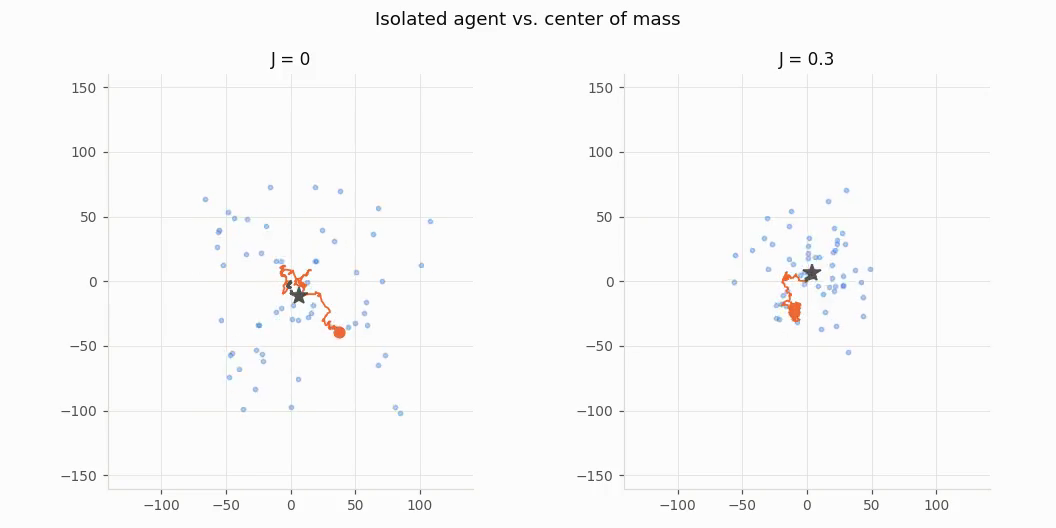
\includegraphics[width=0.65\textwidth]{figs/fig4_meanfield_animation_still.png}
\caption{Frame from the mean-field comparison animation
(\code{results/media/phase3\_figures/fig4\_meanfield\_animation.mp4}),
$N{=}60$, $T{=}400$, $K{=}512$: an isolated agent's trajectory (orange) and
the population's centre of mass (star) against the full population (faint
points). The animation, not reproducible in a static panel, shows the
isolated agent's excursions being visibly damped relative to the spread of
the population as coupling increases from $J{=}0$ to $J{=}0.3$.}
\label{fig:meanfield}
\end{figure}

\clearpage
% =====================================================================
\section{Overall conclusion}
\label{sec:conclusion}

\textbf{Q1 (single-trajectory estimator reliability)} is answered concretely,
not just qualitatively: a single trajectory is unreliable in two distinct
ways depending on the mechanism, and the two look different from the inside.
Scaled Brownian motion converges tightly onto a wrong exponent, so the
estimator's own precision gives no warning; CTRW converges slowly onto a
wrong exponent and keeps a wide, barely-shrinking spread, so at least the
estimator is honest about its own uncertainty. Both report
$\hat\alpha\approx1$ from a single trajectory for unrelated reasons, and that
coincidence is the concrete obstacle Phase 2 exists to remove.

\textbf{Q2 (mechanism discrimination)} is largely solved within the scope
tested: nineteen scale-invariant features, mostly drawn from the propagator
shape and the immobility structure rather than the exponent itself, separate
every mechanism pair tested, several of them (fBm vs.\ CTRW, DDM vs.\
Brownian) almost perfectly even at short trajectory lengths. Once the
mechanism is known, a mechanism-specific correction --- including one built
from first principles for the L\'evy walk, after two more natural approaches
failed for diagnosable reasons --- closes most of the gap to an oracle that
already knows the mechanism.

\textbf{Q3 (single agent vs.\ collective)} has a genuinely asymmetric answer,
and that asymmetry is the phase's central physical finding: coupling
destroys a superdiffusive agent's ability to reveal the collective regime
from its own short-term behaviour, but does not destroy a subdiffusive
agent's ability to do so. The field itself is always informative and its
precision is provably independent of the coupling strength (the conservation
law, confirmed at the level of an estimator's bias and variance, not only in
the field's own spectrum) --- so a field-aware observer is the most reliable
of the four tested at every coupling strength, and a naive, coupling-blind
observer is actively misleading, not merely noisier, once coupling is
non-trivial.

\textbf{Q4 (modular heterogeneity)} remains open: Phase 4 has not been run.
What Phase 3 establishes as its precondition is concrete rather than
aspirational: a validated coupled-agent simulator, an estimator toolbox whose
efficiency is measured (not assumed) against the relevant Cram\'er--Rao
bounds at the scale it was tested ($N{=}400$), and an explicit list of what
is \emph{not} yet known at other scales --- field-aware variance should not
be assumed $N$-independent when budgeting Phase 4 (Table~\ref{tab:n-scaling}
shows a real, unexplained rise with $N$), and wall-clock cost is
super-linear in both $N$ and $K$ with a sharp, localized cost jump once $K$
exceeds a few thousand (Table~\ref{tab:k-scaling}). These are the concrete
numbers Phase 4's design should be budgeted against, not a smooth
extrapolation from the $N{=}400$ scale this report's results were measured
at.

\end{document}
